\documentclass[aspectratio= 169]{beamer}
\usepackage{amsmath}
\usepackage{amssymb}
\usepackage{booktabs}
\usepackage{float}
\usepackage{tikz}
\usetheme{Boadilla}
\usepackage{tikz}
\usepackage{graphics}
\graphicspath{{./Cells}}
\setbeamertemplate{caption}[numbered]

\newcommand{\nb}{\textbf{\textit{NB! }}}
\newcommand{\bi}[1]{\textbf{\textit{#1 }}}
\newcommand{\R}{\mathbb{R}}

\title[Stock returns forecasting]{Neural networks and econometric models in forecasting stock returns}
\author{Andrew~Grishin}

\institute[Faculty of Economics MSU]{Faculty of Economics Moscow State University}
\date{\today}

\begin{document}
	
	\begin{frame}
		\titlepage
	\end{frame}

	\begin{frame}{Agenda}
		\tableofcontents
	\end{frame}

	\section{Problem Formalization}
	\begin{frame}{Problem Formalization}
		
		\begin{columns}[T]
			\begin{column}{.59\textwidth}
				
					Given:
					\begin{enumerate}
						\item Company name.
						\item ${y_t: t = \overline{1, n}}$ - its earning yields series.
					\end{enumerate}
					Aim:
					\begin{enumerate}
						\item To predict the yield in the \textit{next} period of time. 
						\item Mathematical view: ${\mathbb{E} \left(y_{t+1} | y_t, y_{t - 1}, ..., y_1 \right)}$.
					\end{enumerate}
					
				\end{column}%
				\hfill%
				\begin{column}{.32\textwidth}
					History of Methods:
						\begin{enumerate}
							\item Statistics.
							\item Machine Learning.
							\item Deep Learning.
						\end{enumerate}
				\end{column}
			
			\end{columns}

	\end{frame}

	\section{Main Techniques}
	\begin{frame}{Main Techniques}
		Models:
		\begin{enumerate}
			\item \textbf{Decomposition}: deconstruction of time series.
			\item \textbf{Smooth-based}: removal of anomalies.
			\item \textbf{Moving-Average}: tracking a single type of data.
			\item \textbf{Exponential Smoothing}: (2) + exponential window function.
		\end{enumerate}
	\end{frame}

	\section{Already existing solutions}
	\begin{frame}{Already existing solutions}
		Existing solutions for TS forecasting problem:
		
		\begin{columns}[T]
			\begin{column}{0.5\textwidth}
				\begin{enumerate}
					\item Time-series decomposition.
					\item Time-series regression models.
					\item Exponential smoothing (\textbf{EWMA}).
					\item \textbf{ARIMA}, SARIMA, SARIMAX.
					\item \textbf{ARFIMA}, VAR, SVAR.
				\end{enumerate}
			\end{column}
			\hfill
			\begin{column}{0.5\textwidth}
				\begin{enumerate}
					\item (Recurrent) \textbf{Neural Networks}.
					\item \textbf{GARCH}, \textbf{FIGARCH}.
					\item \textbf{SETARMA}, ADL.
					\item \textbf{SVM}, \textbf{SSA}, TBATS.
					\item[] etc.
				\end{enumerate}
			\end{column}
		\end{columns}

	\end{frame}

		\subsection{Stationary methods}
		\begin{frame}{Stationary methods (1)}
			\begin{enumerate}
				
				\item AR(F)IMA(p, d, q) (Autoregressive Fractionally Integrated Moving Average)
				\begin{equation}
					\left(1 - \sum_{i = 1}^p \phi_iL^i \right)\nabla^{d}(y_t - \mu) = \left(1 + \sum_{j = 1}^q \theta_jL^j\right)\varepsilon_t
				\end{equation}
				\begin{columns}[T]
					\begin{column}{0.48\textwidth}
						$${ARIMA \Rightarrow d \in \mathbb{Z}^+}$$
						$${\nabla^d = \left(1 - L\right)^d}$$
					\end{column}
					\hfill
					\begin{column}{0.48\textwidth}
						$${ARFIMA \Rightarrow d \in (-0.5, 0.5)}$$
						$${\nabla^d = \sum_{k = 0}^\infty \frac{\Gamma{(k - d)}L^k}{\Gamma{(-d)} \Gamma{(k + 1)}}}$$
					\end{column}
				\end{columns}
			\end{enumerate}
		\end{frame}
	
		\begin{frame}{Stationary methods (2)}
			\begin{enumerate}
				\item GARCH(p, q)\footnote{Empirically proved that GARCH(1, 1) is better to use in practice.} Conditional Heteroscedasticity:
				\begin{equation}
					\sigma^2_t = \alpha_0 + \sum_{j = 1}^p \alpha_j \varepsilon^2_{t - j} + \sum_{i = 1}^{q} \phi_i \sigma^2_{t - i} = \alpha_0 + \alpha\left(L\right) \varepsilon_t^2 + \beta\left(L\right) \sigma^2_t
				\end{equation}
			
				\item FIGARCH(p, d, q)
				\begin{equation}
					\sigma_t^2 = \alpha_0\left[1 - \beta\left(L\right)\right]^{-1} + \varepsilon_t^2 \left[1 - \left[1 - \beta\left(L\right)\right]^{-1} \cdot \left(1 - L \right)^d \cdot \overbrace{\phi\left(L\right)}^{1 - \alpha\left(L\right) - \beta\left(L\right)}\right]
				\end{equation}
				$${d \in (0, 1)}$$
			\end{enumerate}
		\end{frame}
	
		\begin{frame}{Stationary methods (3)}
			\begin{enumerate}
				\item SETARMA${(k; p_1, \ldots, p_k; q_1, \ldots, q_k)}$ (Self Exciting Threshold ARMA)
				\begin{equation}
					y_t = \sum_{i = 1}^k \left[\phi_0^{(i)} + \overbrace{\Phi^{(i)}\left(L\right)  y_{t}}^{\sum_{j = 1}^{p_i} \phi_j^{(i)} y_{t - j}} + \varepsilon_t - \overbrace{\Theta^{(i)}\left(L\right)\varepsilon_t}^{\sum_{w = 1}^{q_i} \theta_w^{(i)} \varepsilon_{t - w}}\right] \cdot I\left(y_{t - d} \in R_i\right)
				\end{equation}
				$${\varepsilon \sim N\left(0, \sigma^2\right), d - \text{ threshold delay}, I(\cdot) - \text{ Bernoulli random process}}$$
				$${R_i = [r_{i - 1}, r_i): -\infty = r_0 < \ldots < r_{i - 1} < r_i < \dots < r_k = \infty: r_i - \text{ threshold} }$$
				$${\bigcup_{i = 1}^k R_i = \R}$$
				%  
				% 
			\end{enumerate}
		\end{frame}
		
		\subsection{Non Stationary Methods}
			\begin{frame}{Non Stationary Methods (1)}
				\begin{enumerate}
					\item EWMA (Exponential Weighted Moving Average\footnote{$\beta = \frac{2}{n + 1}$: n - number of days for averaging, 2 - smoothing factor.})
					\begin{equation}
						EWMA_t = \frac{v_t}{1 - \beta^t} = \beta \cdot y_{t} + (1 - \beta) \cdot EWMA_{t - 1}
					\end{equation}
					
					\item Neural Networks (sequential adjustment of feature space):
					\begin{equation}
						\varphi_k(W_{k - 1} \cdot \varphi_{k - 1}(W_{k - 2} \cdot (\ldots (W_1 \cdot X) \ldots)))
					\end{equation}
					
					\item SVM - Support Vector Machine Regressor.
					\begin{equation}
						\left\{\begin{array}{l}
							\displaystyle
							\langle w, w \rangle + C \sum_{j = 1}^n \xi_j \rightarrow \min_{w, b}: C \in \R\\
							\displaystyle
							y_j(\langle w, x_j \rangle + b) \ge 1 - \xi_j : \forall j\\
							\displaystyle
							\xi_j \ge 0 : \forall j\\
						\end{array}\right.
					\end{equation}
				\end{enumerate}
			\end{frame}
		
			\begin{frame}{Non Stationary Methods (SSA) (2)}
					Singular Spectrum Analysis (SSA)
					\begin{enumerate}
						\item Turn ${Y = (y_0, ..., y_{N - 1})}$ into Hankel's (trajectory) matrix.
						\begin{equation}
							Y \rightarrow X \in \R^{L, K}: L \in [2, \lfloor N / 2 \rfloor], K = N - L + 1
						\end{equation}
						\item Singular Vector Decomposition (SVD) of Hankelian.
						\begin{equation}
							X = \underbrace{U}_{L \times L} \underbrace{\Sigma}_{L \times K} \underbrace{V^*}_{K \times K}
						\end{equation}
						${d - \textbf{rank}(X)}$.\\
						For orthonormal $V \in \R^{K,K} \Rightarrow V^{-1} = V^T$ and ${V \in \mathbb{C}^{K, K} \Rightarrow V^* = \left(\overline{V}\right)^T}$\\
						${U}$ - \textbf{columns} are performing \textbf{orthonormal basis set} in space of \textbf{columns} in X.\\
						${V}$ - \textbf{columns} are performing \textbf{orthonormal basis set} in space of \textbf{rows} in X.\\
						${\Sigma}$ - "diagonal" matrix composed of singular values of ${XX^T}$, which are equal to ${X^TX}$.
					\end{enumerate}
			\end{frame}
		
			\begin{frame}{Non Stationary Methods (SSA) (3)}
				\begin{enumerate}
					\item $X$ spectral decomposition can be represented:
					\begin{equation}
						X = \sum_{j = 0}^{d - 1} \sigma_j U_j V_j^* = \sum_{j = 0}^{d - 1} \sigma_j \overbrace{U_j}^{L \times 1} \overbrace{V_j^*}^{1 \times K} = \sum_{j = 0}^{d - 1} X_j = \sum_{s \in S} X_s + \sum_{t \in T} X_t + \ldots
					\end{equation}
					$s \in S$ - seasonality. $t \in T$ - trend.\\
					${(\sigma_j, U_j, V_j^*) - \text{ singular triple}: \sigma_j = \sqrt{\lambda_j}}$ - contribution of $j$ elementary matrix to $X$.
					
					\item Reconstruction of Hankel's matrix from $X_j$ elementary matrix by Hankelisation.
					\begin{equation}
						\begin{array}{l}
							\hat{H}: L\times K \rightarrow L \times K\\
							\tilde{X_j} = \hat{H}X_j - \text{ anti-diagonal elements are $\approx$ equal.}\\
							\tilde{X_j} \rightarrow \tilde{Y_j} - \text{ reconstructed $Y$ by anti-diagonal averaging.}
						\end{array}
					\end{equation}
				\end{enumerate}
			\end{frame}
		
			\begin{frame}{Non Stationary Methods (SSA) (4)}
				\begin{equation}
					\begin{array}{lr}
						\hat{H}(A + B) = \hat{H}A + \hat{H}B. & \hat{H}(\alpha A) = \alpha \hat{H}A \Rightarrow \text{Linear Operator.}
					\end{array}
				\end{equation}
				\begin{equation}
					X = \hat{H}X = \hat{H} \left(\sum_{j = 0}^{d - 1} \sigma_j U_j V_j^*\right) = \sum_{j = 0}^{d - 1} \hat{H}X_j = \sum_{j = 0}^{d - 1} \tilde{X}_j
				\end{equation}
				\begin{equation}
					\tilde{x}_{m,n} = 
						\left\{\begin{array}{ll}
							\displaystyle
							\frac{1}{s + 1} \sum_{l = 0}^s x_{l, s - l} & \text{, } 0 \le s \le L - 1\\
							\displaystyle
							\frac{1}{L - 1} \sum_{l = 0}^{L - 1} x_{l, s - l} & \text{, } L \le s \le K - 1\\
							\displaystyle
							\frac{1}{K + L - S - 1} \sum_{l = s - K + 1}^L x_{l, s- l} & \text{, } K \le s \le K + L - 2
						\end{array}\right.
				\end{equation}
				$s = m + n$. We achieve the reconstructed times series from its decomposed parts.
			\end{frame}
			
			\begin{frame}{Non Stationary Methods (SSA) (5)}
				\textbf{Q}: How to determine, which components should be grouped together?\\
				\textbf{A}: Introduce the inner weights.
				\begin{enumerate}
					\item Firstly: inner weighted product (frequency of each element in $\tilde{X}_j$).
					\begin{equation}
						w_k = \left\{\begin{array}{ll}
							k + 1 & \text{, } 0 \le k \le L - 1\\
							L & \text{, } L \le k \le K - 1\\
							N - k & \text{, } K \le k \le N - 1
						\end{array}\right.
					\end{equation}
				
					\item Correlation matrix (there is no noiseless dependences in real world data).
					\begin{equation}
						W_{corr} = \left\{ w_{i, j} = \frac{\left(\tilde{Y}_j, \tilde{Y}_i\right)_w}{\lVert \tilde{Y}_i \rVert_w \lVert \tilde{Y}_j \rVert_w} \right\}_{i, j = 0}^{N - 1}: \left(\tilde{Y}_j, \tilde{Y}_i\right)_w = \sum_{k = 0}^{N - 1} w_k \cdot \tilde{y}_{i, k} \cdot \tilde{y}_{j, k}
					\end{equation}
				\end{enumerate}
				$w_{i, j} \rightarrow 1$ if components $\tilde{Y}_i$ and $\tilde{Y}_j$ are close, else $w_{i, j} \rightarrow 0$.\\ In practice is $w_{i, j} \ge 0.3 \Rightarrow \tilde{Y}_i$ and $\tilde{Y}_j$ should be grouped together.
			\end{frame}
		
			\begin{frame}{Non Stationary Methods (SSA) (6)}
				Forecasting algorithm:\\
				\textbf{Note:} ${U_j}$ - $j$ column of $U$.
				\begin{enumerate}
					\item Count ${r = \lvert \left\{\sigma_j: \sigma_j > 0 \right\} \rvert}$.
					\item Take ${\left\{ \underline{U}_{j, k} : 1 \le j \le r, 1 \le k < L \right\}: U}$ -  matrix of orthonormal column-vectors.
					\item Take ${\left\{\pi_j : \pi_j = U_{j, L}: j = \overline{1, r}\right\}}$ - ${\pi_j}$ - the last element of each of $r$ columns in matrix $U$.
					\item Evaluate $\nu = \sum_{j = 1}^r \pi_j^2$.
					\item Compute vector of coefficients ${R = \left(a_{L - 1}, \ldots, a_{1}\right)^T = \frac{1}{1 - \nu} \sum_{j = 1}^r \pi_j \underline{U}_j}: \underline{U}_j \in \R^{L-1, 1}$
					\item Evaluate the forecast formula:
					\begin{equation}
						y_t = 
						\left\{\begin{array}{ll}
							\displaystyle
							\tilde{y}_t & \text{, } t = \overline{1, N}\\
							\displaystyle
							\sum_{j = 1}^{L - 1}a_j y_{t - j} & \text{, } t = \overline{N+1, N + h}
						\end{array}\right.
					\end{equation}
				\end{enumerate}
			${\tilde{y}_t}$ - reconstructed TS without noise components.
			\end{frame}
	
	\section{RNN}
		\subsection{Simple RNN}
		\begin{frame}{Simple RNN\footnote{Do not look at bidirectional way.} (1)}
			\begin{itemize}
				\item Simple RNN block\footnote{Usually $h_0$ is initialized with $\textbf{0}$.} specified for our problem:
				
				
				\begin{columns}[T]
					\begin{column}{0.45\textwidth}
						$${
							\begin{array}{l}
								h_t = \tanh{\left( W_{hh} h_{t - 1} + b_{hh} + W_{hx} x_t + b_{hx} \right)}\\
								W_{hx} \in \R^{H_{out} \times H_{in}}, x_t \in \R^{ H_{in} \times 1}\\
								W_{hh} \in \R^{H_{out} \times H_{out}}, h_{t} \in \R^{H_{out} \times 1}\\
								b_{hx}, b_{hh} \in \R^{H_{out} \times 1}
							\end{array}
						}$$
					\end{column}
					\hfill
					\begin{column}{0.45\textwidth}
						\begin{figure}[H]
							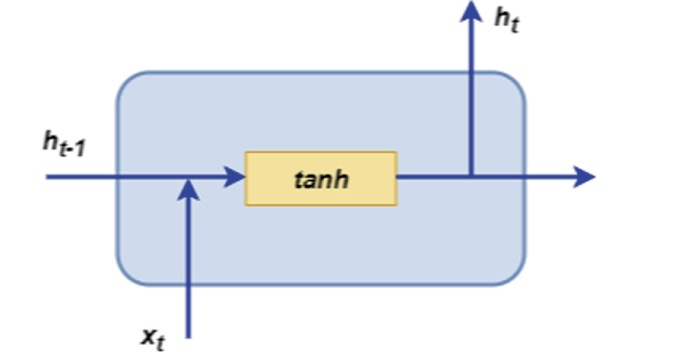
\includegraphics[width= 5cm, height= 3cm]{RNN_cell.jpg}
							\caption{Simple RNN cell}
						\end{figure}
					\end{column}
				\end{columns}				
			\end{itemize}
		\end{frame}
	
		\subsection{GRU}
		\begin{frame}{Gate Recurrent Unit}
			\begin{itemize}
				\item GRU:
					\begin{columns}[T]
						\begin{column}{0.45\textwidth}
							$${
								\begin{array}{l}
									r_t = \sigma\left(W_{ir} x_t + b_{ir} + W_{hr}h_{t-1} + b_{hr}\right)\\
									z_t = \sigma\left(W_{iz}x_t + b_{iz} + W_{hz}h_{t - 1} + b_{hz}\right)\\
									n_t = \tanh\left(W_{in} x_t + b_{in} + r_t * \left({W_{hn}h_{t - 1} + b_{hn}}\right)\right)\\
									h_t = (1 - z_t) * n_t + z_t * h_{t - 1}
								\end{array}
							}$$
						\end{column}
						\hfill
						\begin{column}{0.45\textwidth}
							\begin{figure}[H]
								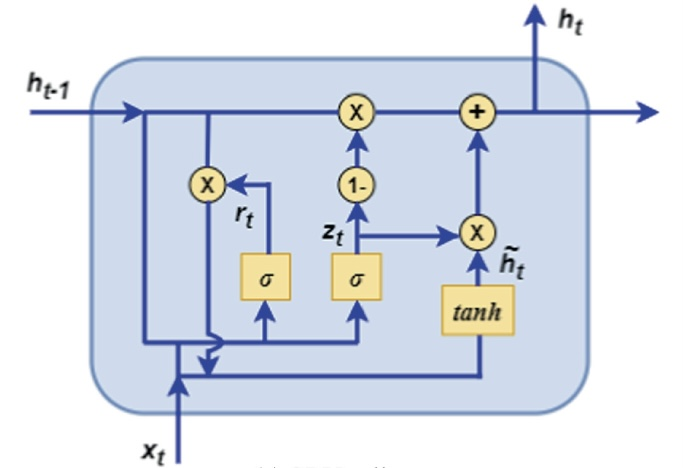
\includegraphics[width= 4.5cm, height= 3cm]{GRU_cell.jpg}
								\caption{GRU cell}
							\end{figure}
						\end{column}
					\end{columns}
			\end{itemize}
		\end{frame}
	
		\subsection{LSTM}
		\begin{frame}{Long-Short Term Memory}
			\begin{itemize}
				\item LSTM:
				\begin{columns}
					\begin{column}{0.45\textwidth}
						$${
							\begin{array}{l}
								i_t = \sigma\left(W_{ii}x_t + b_{ii} + W_{hi}h_{t - 1} + b_{hi}\right)\\
								f_t = \sigma\left(W_{if}x_t + b_{if} + W_{hf} h_{t - 1} + b_{hf}\right)\\
								g_t = \tanh\left( W_{ig}x_t + b_{ig} + W_{hg}h_{t - 1} + b_{hg} \right)\\
								o_t = \sigma\left(W_{io}x_t + b_{io} + W_{ho}h_{t - 1} + b_{ho}\right)\\
								c_t = f_t * c_{t - 1} + i_t * g_t\\
								h_t  = o_t * \tanh\left(c_t\right)
							\end{array}
						}$$
					\end{column}
					\hfill
					\begin{column}{0.45\textwidth}
						\begin{figure}[H]
							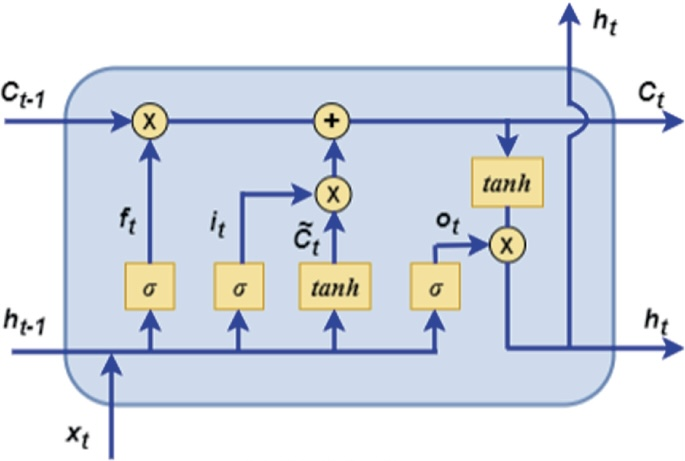
\includegraphics[width= 4.5cm, height= 3cm]{LSTM_cell.jpg}
							\caption{LSTM cell}
						\end{figure}
					\end{column}
				\end{columns}
					
			\end{itemize}
		\end{frame}
	
	\section{Comparison of results}
	\begin{frame}{Comparison of results}
		content...
	\end{frame}

	\section{Conclusion}
	\begin{frame}{Conclusion}
		content...
	\end{frame}

	\begin{frame}
		\centering
		\LARGE
		Thank you for attention!
	\end{frame}
	
\end{document}